%definira klasu dokumenta 
\documentclass[12pt]{report} 

%prostor izmedu naredbi \documentclass i \begin{document} se zove uvod. U njemu se nalaze naredbe koje se odnose na cijeli dokument

%osnovni LaTex ne može riješiti sve probleme, pa se koriste različiti paketi koji olakšavaju izradu željenog dokumenta
\usepackage[croatian]{babel} 
\usepackage{amssymb}
\usepackage{amsmath}
\usepackage{txfonts}
\usepackage{mathdots}
\usepackage{titlesec}
\usepackage{array}
\usepackage{lastpage}
\usepackage{etoolbox}
\usepackage{longtable, tabu}
\usepackage{color, colortbl}
\usepackage{adjustbox}
\usepackage{geometry}
\usepackage[classicReIm]{kpfonts}
\usepackage{hyperref}
\usepackage{fancyhdr}
\usepackage{caption}
\usepackage{comment}

\usepackage{float}
\usepackage{setspace}
\restylefloat{table}


\patchcmd{\chapter}{\thispagestyle{plain}}{\thispagestyle{fancy}}{}{} %redefiniranje stila stranice u paketu fancyhdr

%oblik naslova poglavlja
\titleformat{\chapter}{\normalfont\huge\bfseries}{\thechapter.}{20pt}{\Huge}
\titlespacing{\chapter}{0pt}{0pt}{40pt}


\linespread{1.3} %razmak između redaka

\geometry{a4paper, left=1in, top=1in,}  %oblik stranice

\hypersetup{ colorlinks, citecolor=black, filecolor=black, linkcolor=black,	urlcolor=black }   %izgled poveznice


%prored smanjen između redaka u nabrajanjima i popisima
\newenvironment{packed_enum}{
	\begin{enumerate}
		\setlength{\itemsep}{0pt}
		\setlength{\parskip}{0pt}
		\setlength{\parsep}{0pt}
	}{\end{enumerate}}

\newenvironment{packed_item}{
	\begin{itemize}
		\setlength{\itemsep}{0pt}
		\setlength{\parskip}{0pt}
		\setlength{\parsep}{0pt}
	}{\end{itemize}}


%boja za privatni i udaljeni kljuc u tablicama
\definecolor{LightBlue}{rgb}{0.9,0.9,1}
\definecolor{LightGreen}{rgb}{0.9,1,0.9}


%podesavanje zaglavlja i podnožja

\pagestyle{fancy}
\lhead{Programsko inženjerstvo}
\rhead{$Pomozi $\space$ mi$}
\lfoot{$NULL$}
\cfoot{stranica \thepage/\pageref{LastPage}}
\rfoot{\today}
\renewcommand{\headrulewidth}{0.2pt}
\renewcommand{\footrulewidth}{0.2pt}


\begin{document} 
	
	
	
	\begin{titlepage}
		\begin{center}
			\vspace*{\stretch{1.0}} %u kombinaciji s ostalim \vspace naredbama definira razmak između redaka teksta
			\LARGE Programsko inženjerstvo\\
			\large Ak. god. 2020./2021.\\
			
			\vspace*{\stretch{3.0}}
			
			\huge $ Pomozi $\space$ mi $\\
			\Large Dokumentacija, Rev. \textit{$1$}\\
			
			\vspace*{\stretch{12.0}}
			\normalsize
			Grupa: \textit{$NULL$}\\
			Voditelj: \textit{Iva \space Bokšić}\\
			
			
			\vspace*{\stretch{1.0}}
			Datum predaje: \textit{12. 11. $2020$.}\\
	
			\vspace*{\stretch{4.0}}
			
			Nastavnik: \textit{$Dunja $\space$ Tounec$}\\
		
		\end{center}

	
	\end{titlepage}

	
	\tableofcontents

	\chapter{Dnevnik promjena dokumentacije}
		
		\textbf{\textit{Kontinuirano osvježavanje}}\\
				
		
		\begin{longtabu} to \textwidth {|X[2, l]|X[13, l]|X[3, l]|X[3, l]|}
			\hline \multicolumn{1}{|l|}{\textbf{Rev.}}	& \multicolumn{1}{l|}{\textbf{Opis promjene/dodatka}} & \multicolumn{1}{|l|}{\textbf{Autori}} & \multicolumn{1}{l|}{\textbf{Datum}} \\[3pt] \hline
			\endfirsthead
			
			\hline \multicolumn{1}{|l|}{\textbf{Rev.}}	& \multicolumn{1}{l|}{\textbf{Opis promjene/dodatka}} & \multicolumn{1}{|l|}{\textbf{Autori}} & \multicolumn{1}{l|}{\textbf{Datum}} \\[3pt] \hline
			\endhead
			
			\hline 
			\endlastfoot
			
			0.1 & Napravljen predložak.	& Ivošević & 22.08.2013. 		\\[3pt] \hline 
			0.2	& Dopisane upute za povijest dokumentacije.\newline Dodane reference. & Jović & 24.08.2013. 	\\[3pt] \hline 
			0.5 & Dodan \textit{Use Case} dijagram i jedan sekvencijski dijagram, funkcionalni i nefunkcionalni zahtjevi i dodatak A & Ivošević & 25.08.2013. \\[3pt] \hline 
			0.6 & Arhitektura i dizajn sustava, algoritmi i strukture podataka & Grudenić & 26.08.2013. \\[3pt] \hline 
			0.8 & Povijest rada i trenutni status implementacije,\newline Zaključci i plan daljnjeg rada & Ivošević & 28.08.2013. \\[3pt] \hline 
			0.9 & Opisi obrazaca uporabe & Jović & 07.09.2013. \\[3pt] \hline 
			0.10 & Preveden uvod & Jović & 08.09.2013. \\[3pt] \hline 
			0.11 & Sekvencijski dijagrami & Žužak & 09.09.2013. \\[3pt] \hline 
			0.12.1 & Započeo dijagrame razreda & Horvat & 10.09.2013. \\[3pt] \hline 
			0.12.2 & Nastavak dijagrama razreda & Horvat & 11.09.2013. \\[3pt] \hline 
			\textbf{1.0} & Verzija samo s bitnim dijelovima za 1. ciklus & Ivošević & 11.09.2013. \\[3pt] \hline 
			1.1 & Uređivanje teksta -- funkcionalni i nefunkcionalni zahtjevi & Grudenić \newline Jović & 14.09.2013. \\[3pt] \hline 
			1.2 & Manje izmjene:Timer - Brojilo vremena & Grudenić & 15.09.2013. \\[3pt] \hline 
			1.3 & Popravljeni dijagrami obrazaca uporabe & Jović & 15.09.2013. \\[3pt] \hline 
			1.5 & Generalna revizija strukture dokumenta & Ivošević & 19.09.2013. \\[3pt] \hline 
			1.5.1 & Manja revizija (dijagram razmještaja) & Jović & 20.09.2013. \\[3pt] \hline 
			\textbf{2.0} & Konačni tekst predloška dokumentacije  & Ivošević & 28.09.2013. \\[3pt] \hline 
			&  &  & \\[3pt] \hline
			
			
		\end{longtabu}
	
	
		\textit{Moraju postojati glavne revizije dokumenata 1.0 i 2.0 na kraju prvog i drugog ciklusa. Između tih revizija mogu postojati manje revizije već prema tome kako se dokument bude nadopunjavao. Očekuje se da nakon svake značajnije promjene (dodatka, izmjene, uklanjanja dijelova teksta i popratnih grafičkih sadržaja) dokumenta se to zabilježi kao revizija. Npr., revizije unutar prvog ciklusa će imati oznake 0.1, 0.2, …, 0.9, 0.10, 0.11.. sve do konačne revizije prvog ciklusa 1.0. U drugom ciklusu se nastavlja s revizijama 1.1, 1.2, itd.}
	\chapter{Opis projektnog zadatka}
		
		\textbf{\textit{dio 1. revizije}}\\
		
		\textit U okviru projekta za razvoj programske potpore cilj nam je napraviti web aplikaciju 
“Pomozi mi“ čiji je primarni zadatak mogućnost traženja pomoći te pružanje same usluge od strane ljudi koji žele pomagati. Potencijalna korist mogla bi biti i samo zbližavanje korisnika te širenje osjećaja sigurnosti i povezanosti same zajednice. Na ovaj način mnogi ljudi kojima je odlazak u trgovinu ili košnja trave veliki izazov pronalaze način da dođu do osoba koji svoj višak vremena žele iskoristiti za pomaganje potrebitijima. Iako danas postoje mnoge društvene mreže, ova stranica nema nepotreban sadržaj te je maksimalno prilagođena svojoj funkciji uz jednostavno korištenje. \newline
Prvi korak prema korištenju usluga same aplikacije je prijava u sustav.
Svaki korisnik aplikacije ukoliko nema otvoreni profil (javni korisnik) se mora registrirati. Prilikom registracije ostavlja osnovne podatke o sebi :

		\begin{packed_item}
			\item \textit Ime
			\item \textit Prezime
			\item \textit Lozinka
			\item \textit Adresa
			\item \textit e-mail
		\end{packed_item}
		
		\textit Za svako sljedeće korištenje dovoljna je prijava pomoću e-mail adrese i lozinke.

Nakon prijave korisnik može pristupiti pregledu svog profila, listi korisnika ili odabrati neku od dvije aktivnosti same aplikacije: nudi li pomoć ili je traži te s obzirom na odabir se otvara odgovarajuća stranica. 

		\eject

		%unos slike
		\begin{figure}[H]
			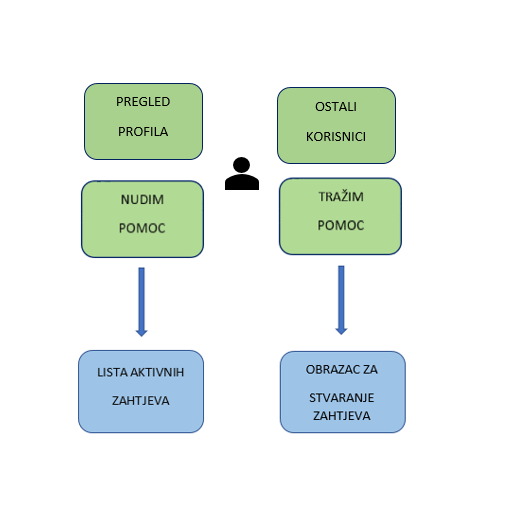
\includegraphics[scale=0.6]{slike/projekt1.png} %veličina slike u odnosu na originalnu datoteku i pozicija slike
			\centering
			\caption {odabir nakon prijave}
			\label{fig:promjene}
		\end{figure}
		
		\textit Kada korisnik traži pomoć ispunjava obrazac za stvaranje zahtijeva. Na njemu unosi sljedeće podatke:
		
		\begin{packed_item}
			\item \textit Kratki opis posla
			\item \textit Kontakt: broj mobitela / e-mail
			\item \textit Opcionalno datum i vrijeme
			\item \textit Opcionalno lokacija
		\end{packed_item}

        \textit Ukoliko je lokacija važna za izvršavanje usluge može se dohvatiti s uređaja ili označiti na karti.
        \newline
Nakon objave korisnik je autor zahtjeva te je u mogućnosti zahtjev obrisati trajno iz baze podataka ili ga trenutno blokirati. Objavljeni zahtjev se nalazi na listi aktivnih zahtjeva.
\newline
Svi koji žele pomoći, na stranici aktivnih zahtjeva pronalaze koju uslugu bi mogli izvršiti. Prilikom pregleda liste moguće je lako dohvatiti profil korisnika koji je objavio zahtjev.Svakom korisniku se prikazuju samo zahtjevi čija je lokacija unutar jednog kilometra od uređaja korisnika te zahtjevi za čije je izvršavanje lokacija nebitna. Kada korisnik pronađe zadovoljavajuću ponudu usluge odabire izvršavanje čime postaje izvršitelj zahtjeva.

        		%unos slike
		\begin{figure}[H]
			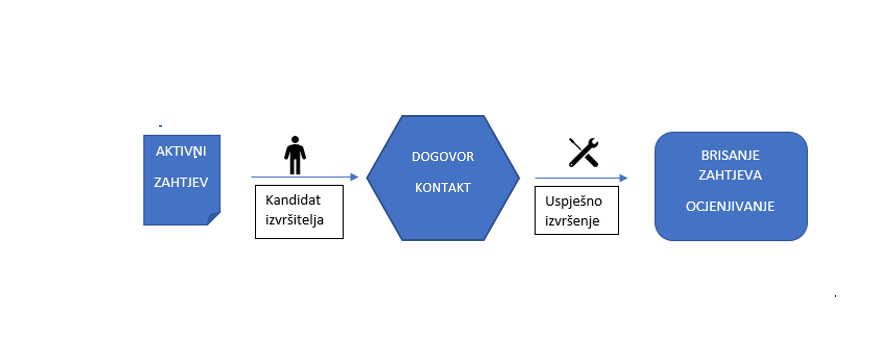
\includegraphics[scale=0.7]{slike/projekt2.png} %veličina slike u odnosu na originalnu datoteku i pozicija slike
			\centering
			\caption {proces izvršavanja zahtjeva}
			\label{fig:promjene}
		\end{figure}

        \textit Odabirom posla šalje se automatska obavijest autoru zahtjeva o potencijalnom izvršitelju. Izvršitelj i autor mogu dodatno pojasniti sam posao i ostale detalje izvedbe. Nakon što je usluga obavljena autor zahtjev označava kao izvršen te se briše s liste aktivnih.  
        \newline
Nakon izvršenja posla moguće je ocijeniti drugog korisnika ocjenama 1-5 te ostaviti komentar. Ocjenjivanje je moguće i kad si korisnici nisu međusobno pomagali, a sve ocjene i komentari su vidljivi na profilu korisnika.
        \newline
Svaki korisnik svoj profil može vidjeti u svakom trenutku, a ostale korisnike može pretražiti ili ih dohvatiti među aktivnim zahtjevi. Na tuđim profilima su vidljivi :
		
		\begin{packed_item}
			\item \textit Ime
			\item \textit Prezime
			\item \textit Ocjene i komentari drugih korisnika
			\item \textit "lanac povjerenja"

		\end{packed_item}
		
		
“Lanac povjerenja“ prikazuje kako su ljudi koje sami ocijenimo visoko ocijenili profil koji trenutno gledamo. Na taj način korisnik se sigurnije osjeća za daljnju komunikaciju s korisnikom profila.
\newline
Kada korisnik gleda vlastiti profil ima mogućnost pristupa listi vlastitih zahtjeva. Unutar liste vlastitih zahtjeva bira pregled izvršenih ili aktivnih kojima može dodatno upravljati. Zahtjevi su sortirani vremenski, a moguće su još dodatne opcije filtriranja poput kategorije i lokacije. Svi zahtjevi koji su aktivni, izvršeni ili blokirani ostaju pohranjeni u bazi podataka.
\newline

Osim korisnika važnu ulogu imaju administratori koji su dodijeljeni za određenu geografsku lokaciju. Oni brinu da sadržaj koji se objavljuje ne bude lažan ili opasan te imaju mogućnost brisanja zahtjeva i profila. Oni mogu privremeno ili trajno blokirati sve korisnike aplikacije.
\newline
Ova aplikacija se lako po potrebi može proširiti i na druga područja uz male preinake vrsta zahtjeva. Također ukoliko se uoči potreba moguće je lako stvoriti i mobilnu aplikaciju koja bi još dodatno olakšala sam pristup korisnicima.

\eject
		
	
	\chapter{Specifikacija programske potpore}

\section{Funkcionalni zahtjevi}

\textbf{\textit{dio 1. revizije}}\\



\noindent \textbf{Dionici:}

\begin{packed_enum}
	
	\item Razvojni tim
	\item Administrator			
	\item Korsinik
	\item Vanjski suradnici - CROZ
	
\end{packed_enum}

\noindent \textbf{Aktori i njihovi funkcionalni zahtjevi:}


\begin{packed_enum}
	\item  \underbar{Korisnik (inicijator) može:}
	
	\begin{packed_enum}
		
		\item poprimiti ulogu autora zahtjeva 
		\begin{packed_enum}
			
			\item   može zadati zahtjev za pomoć
			\item  može obrisati ili blokirati unešeni zahtjev
			
		\end{packed_enum}
		\item poprimiti ulogu izvršitelja zahtjeva 
		\begin{packed_enum}
			
			\item  može odabrati zahtjev s liste aktivnih zahtjeva
			
		\end{packed_enum}
		
		\item razmjenjivati notifikacije kada izvršitelj odabere zahtjev
		\item dohvatiti profil drugog korisnika u trenutku pregleda zahtjeva
		\item ocjenjivati i komentirati druge korisnike
		\item vidjeti "lanac povjerenja"
		\item pregledati listu svojih izvršenih i ponuđenih zahtjeva 
	\end{packed_enum}
	
	\item  \underbar{Administrator (inicijator) može:}
	
	\begin{packed_enum}
		
		\item kontrolirati sadržaj koji se objavljuje
		\item brisanje zahtjeva
		\item blokiranje korisnika pristupu aplikaciji 
	\end{packed_enum}
	
	\item  \underbar{Baza podataka (sudionik) može:}
	\begin{packed_enum}
		
		\item spremanje podataka o profilima, zahtjevima, razmjeni notifikacija
		
	\end{packed_enum}
	
	\item  \underbar{Poslužitelj (sudionik) može:}
	\begin{packed_enum}
		
		\item spremanje podataka o profilima, zahtjevima, razmjeni notifikacija
		
	\end{packed_enum}
\end{packed_enum}

\eject 



\subsection{Obrasci uporabe}

\textbf{\textit{dio 1. revizije}}

\subsubsection{Opis obrazaca uporabe}
\textit{Funkcionalne zahtjeve razraditi u obliku obrazaca uporabe. Svaki obrazac je potrebno razraditi prema donjem predlošku. Ukoliko u nekom koraku može doći do odstupanja, potrebno je to odstupanje opisati i po mogućnosti ponuditi rješenje kojim bi se tijek obrasca vratio na osnovni tijek.}\\


\noindent \underbar{\textbf{UC1 - Registracija}}
\begin{packed_item}
	\item \textbf{Glavni sudionik: } Javni korisnik
	\item  \textbf{Cilj:} Stvoriti korisnički račun za pristup sustavu
	\item  \textbf{Sudionici:} Baza podataka
	\item  \textbf{Preduvjet:} -
	\item  \textbf{Opis osnovnog tijeka:}
	
	\item[] \begin{packed_enum}
		
		\item Korisnik odabire opciju za registraciju
		\item Korisnik unosi potrebne korisničke podatke
		\item Korsinik prima obavijest o uspješnoj registraciji
	\end{packed_enum}
	
	\item  \textbf{Opis mogućih odstupanja:}
	
	\item[] \begin{packed_item}
		
		\item[2.a] Odabir već zauzetog korisničkog imena i/ili e-maila, unos korisničkog podatka u nedozvoljenom formatu ili unos neispravnoga e-maila 
		\item[] \begin{packed_enum}
			
			\item Sustav obaviještava korisnika o neispravnom unosu i ponovno ga vraća na stranicu za registraciju
			\item Korisnik mijenja potrebne podatke i završava unos ili odustaje od registracije
			
		\end{packed_enum}
	\end{packed_item}
\end{packed_item}

\noindent \underbar{\textbf{UC2 -Prijava}}
\begin{packed_item}
	\item \textbf{Glavni sudionik: }Registrirani korisnik
	\item  \textbf{Cilj:} Dobiti pristup korisničkom sučelju
	\item  \textbf{Sudionici:} Baza podataka
	\item  \textbf{Preduvjet:} Registracija
	\item  \textbf{Opis osnovnog tijeka:}
	
	\item[] \begin{packed_enum}
		
		\item Unos korisničkog imena i lozinke
		\item Potvrda o ispravnosti unesenih podataka
		\item Pristup korisničkim funkcijama
	\end{packed_enum}
	
	\item  \textbf{Opis mogućih odstupanja:}
	
	\item[] \begin{packed_item}
		
		\item[1.a] Neispravan unos korisničkog imena ili lozinke
		\item[] \begin{packed_enum}
			
			\item sustav obaviještava korisnika o neispravnom unosu i ponovno ga vraća na stranicu za prijavu
			
		\end{packed_enum}
	\end{packed_item}
\end{packed_item}

\noindent \underbar{\textbf{UC3 -Zadavanje zahtjeva za pomoć}}
\begin{packed_item}
	\item \textbf{Glavni sudionik: } Registrirani korisnik
	\item  \textbf{Cilj:} Kreirati novi zahtjev za pomoć
	\item  \textbf{Sudionici:} Baza podataka
	\item  \textbf{Preduvjet:} Korisnik je prijavljen u sustav
	\item  \textbf{Opis osnovnog tijeka:}
	
	\item[] \begin{packed_enum}
		
		\item Korisnik odabire opciju da traži pomoć
		\item Pojavljuje se obrazac za kreiranje zahtjeva za pomoći
		\item Korisnik odabire opciju "Objavi zahtjev"
	\end{packed_enum}
\end{packed_item}
\noindent \underbar{\textbf{UC3.1 - Određivanje lokacije uređaja}}
\begin{packed_item}
	\item \textbf{Glavni sudionik: } Servis za lociranje uređaja
	\item  \textbf{Cilj:} Dohvatiti trenutnu lokaciju korisnika
	\item  \textbf{Sudionici:} Registrirani korisnik
	\item  \textbf{Preduvjet:} Korisnik je prijavljen u sustav, zadaje se zahtjev za pomoć
	\item  \textbf{Opis osnovnog tijeka:}
	
	\item[] \begin{packed_enum}
		
		\item Korisnik omogućava aplikaciji pristup vlastitoj lokaciji
		\item Korisnik potvrđuje očitanu lokaciju
		\item Očitana lokacija se sprema u bazu
	\end{packed_enum}
	\item  \textbf{Opis mogućih odstupanja:}
	
	\item[] \begin{packed_item}
		
		\item[1.a] Korsnik ne odobrava pristup njegovoj lokaciji, ona nije dostupna ili je krivo očitana
		\item[] \begin{packed_enum}
			
			\item Aplikacija nudi opciju postavljanja lokacije pomoću karte
			
		\end{packed_enum}
	\end{packed_item}
\end{packed_item}
\noindent \underbar{\textbf{UC3.2 - Zadavanje lokacije pomoću karte}}
\begin{packed_item}
	
	\item \textbf{Glavni sudionik: } Servis karte
	\item  \textbf{Cilj:} Postaviti željenu lokaciju pomoću karte
	\item  \textbf{Sudionici:} Registrirani korisnik
	\item  \textbf{Preduvjet:} Korisnik je prijavljen u sustav, zadaje se zahtjev za pomoć
	\item  \textbf{Opis osnovnog tijeka:}
	
	\item[] \begin{packed_enum}
		
		\item Korisnik odabire opciju postavljanja lokacije pomoću karte
		\item Servis karte dohvaća kartu te korisnik precizno odabire željeno područje
		\item Odabrana lokacija se sprema u bazu
	\end{packed_enum}
\end{packed_item}
\noindent \underbar{\textbf{UC4 - Pregled liste korisnika}}
\begin{packed_item}
	
	\item \textbf{Glavni sudionik: }Registrirani korisnik, administrator
	\item  \textbf{Cilj:} Pregledati listu registriranih korisnika
	\item  \textbf{Sudionici:} Baza podataka
	\item  \textbf{Preduvjet:} Korisnik je prijavljen u sustav
	\item  \textbf{Opis osnovnog tijeka:}
	
	\item[] \begin{packed_enum}
		
		\item Korisnik/administrator u bilo kojem trenutku, pritiskom na gumb može pretražiti registrirane korisnike
		\item Iz baze se dohvaća lista profila korisnika
	\end{packed_enum}
\end{packed_item}
\noindent \underbar{\textbf{UC4.1 - Administratorski pregled liste korisnika}}
\begin{packed_item}
	
	\item \textbf{Glavni sudionik: }Administrator
	\item  \textbf{Cilj:} Pregledati listu registriranih korisnika
	\item  \textbf{Sudionici:} Baza podataka
	\item  \textbf{Preduvjet:} Korisnik je prijavljen kao administrator
	\item  \textbf{Opis osnovnog tijeka:}
	
	\item[] \begin{packed_enum}
		
		\item Administrator u bilo kojem trenutku, pritiskom na gumb može pretražiti registrirane korisnike
		\item Iz baze se dohvaća lista profila korisnika
	\end{packed_enum}
\end{packed_item}

\noindent \underbar{\textbf{UC4.2 - Korisnički pregled liste korisnika}}
\begin{packed_item}
	
	\item \textbf{Glavni sudionik: }Registrirani korisnik
	\item  \textbf{Cilj:} Pregledati listu registriranih korisnika
	\item  \textbf{Sudionici:} Baza podataka
	\item  \textbf{Preduvjet:} Korisnik je prijavljen
	\item  \textbf{Opis osnovnog tijeka:}
	
	\item[] \begin{packed_enum}
		
		\item Korisnik u bilo kojem trenutku, pritiskom na gumb može pretražiti registrirane korisnike
		\item Iz baze se dohvaća lista profila korisnika
	\end{packed_enum}
\end{packed_item}

\noindent \underbar{\textbf{UC5 - Prikaz liste aktivnih zahtjeva}}
\begin{packed_item}
	
	\item \textbf{Glavni sudionik: }Registrirani korisnik, administrator
	\item  \textbf{Cilj:} pregledati aktivne zahtjeve i ponuditi pomoć
	\item  \textbf{Sudionici:} Baza podataka
	\item  \textbf{Preduvjet:} Korisnik je prijavljen u sustav
	\item  \textbf{Opis osnovnog tijeka:}
	
	\item[] \begin{packed_enum}
		
		\item Korisnik odabire ulogu izvršitelja zahtjeva
		\item Iz baze se dohvaća lista aktivnih zahtjeva autora koji trebaju pomoć te se nalaze unutar jednog kilometra od lokacije izvršitelja
	\end{packed_enum}
	
	\item  \textbf{Opis mogućih odstupanja:}
	
	\item[] \begin{packed_item}
		
		\item[2.a] Ne postoje aktivni zahtjevi u označenom području
		\item[] \begin{packed_enum}
			
			\item Otvara se mogućnost proširenja liste na veće geografsko područje
			
		\end{packed_enum}
	\end{packed_item}
\end{packed_item}
\noindent \underbar{\textbf{UC5.1 - Administratorski prikaz liste aktivnih zahtjeva}}
\begin{packed_item}
	
	\item \textbf{Glavni sudionik: }Administrator
	\item  \textbf{Cilj:} Pregledati aktivne zahtjeve
	\item  \textbf{Sudionici:} Baza podataka
	\item  \textbf{Preduvjet:} Korisnik je prijavljen kao administrator
	\item  \textbf{Opis osnovnog tijeka:}
	
	\item[] \begin{packed_enum}
		
		\item Administrator odabire opciju pregleda liste aktivnih zahtjeva
		\item Iz baze se dohvaća lista aktivnih zahtjeva autora koji trebaju pomoć te se nalaze unutar jednog kilometra od lokacije administratora
	\end{packed_enum}
	
	\item  \textbf{Opis mogućih odstupanja:}
	
	\item[] \begin{packed_item}
		
		\item[2.a] Ne postoje aktivni zahtjevi u označenom području
		\item[] \begin{packed_enum}
			
			\item Otvara se mogućnost proširenja liste na veće geografsko područje
			
		\end{packed_enum}
	\end{packed_item}
\end{packed_item}
\noindent \underbar{\textbf{UC5.2 - Korisnički prikaz liste aktivnih zahtjeva}}
\begin{packed_item}
	
	\item \textbf{Glavni sudionik: }Registrirani korisnik
	\item  \textbf{Cilj:} Pregledati aktivne zahtjeve i ponuditi pomoć
	\item  \textbf{Sudionici:} Baza podataka
	\item  \textbf{Preduvjet:} Korisnik je prijavljen u sustav
	\item  \textbf{Opis osnovnog tijeka:}
	
	\item[] \begin{packed_enum}
		
		\item Korisnik odabire ulogu izvršitelja zahtjeva
		\item Korisnik odabire opciju pregleda aktivnih zahtjeva
		\item Iz baze se dohvaća lista aktivnih zahtjeva autora koji trebaju pomoć te se nalaze unutar jednog kilometra od lokacije izvršitelja
	\end{packed_enum}
	
	\item  \textbf{Opis mogućih odstupanja:}
	
	\item[] \begin{packed_item}
		
		\item[2.a] Ne postoje aktivni zahtjevi u označenom području
		\item[] \begin{packed_enum}
			
			\item Otvara se mogućnost proširenja liste na veće geografsko područje
			
		\end{packed_enum}
	\end{packed_item}
\end{packed_item}

\noindent \underbar{\textbf{UC6 - Dodjela administrativnog područja}}
\begin{packed_item}
	\item \textbf{Glavni sudionik: }Administrator
	\item  \textbf{Cilj:} dodjela administrativnog područja prema geografskoj lokaciji
	\item  \textbf{Sudionici:} Sustav
	\item  \textbf{Preduvjet:} Korisnik je registriran i prijavljen kao administrator
	\item  \textbf{Opis osnovnog tijeka:}
	
	\item[] \begin{packed_enum}
		
		\item Administratoru preko vlastite lokacije sustav dodjeljuje administrativno područje
	\end{packed_enum}
\end{packed_item}

\noindent \underbar{\textbf{UC7 - Razmjena notifikacija}}
\begin{packed_item}
	
	\item \textbf{Glavni sudionik: } Registrirani korisnik
	\item  \textbf{Cilj:} Dogovor oko izvršavanja zahtjeva
	\item  \textbf{Sudionici:} Baza podataka
	\item  \textbf{Preduvjet:} Korisnik je prijavljen u sustav, korisnik je odabrao zahtjev za izvršavanje
	\item  \textbf{Opis osnovnog tijeka:}
	
	\item[] \begin{packed_enum}
		
		\item Nakon odabira zahtjeva kojeg korisnik želi izvršiti omogućuje se razmjena notifikacija radi dogovora oko izvršenja zahtjeva 
		
	\end{packed_enum}
	
\end{packed_item}

\noindent \underbar{\textbf{UC8 - Ocjenjivanje}}
\begin{packed_item}
	
	\item \textbf{Glavni sudionik: } Registrirani korisnik
	\item  \textbf{Cilj:} Ocjenjivanje korisnika kako bi drugi korisnici vidjeli ukupnu ocjenu  
	\item  \textbf{Sudionici:} Baza podataka
	\item  \textbf{Preduvjet:} Korisnik je prijavljen u sustav
	\item  \textbf{Opis osnovnog tijeka:}
	
	\item[] \begin{packed_enum}
		
		\item Korisnik odabire opciju za ocjenjivanje između 1 i 5
		\item Pohranjuje se dodjeljena ocjena u bazu podataka
	\end{packed_enum}
	
\end{packed_item}

\noindent \underbar{\textbf{UC8.1 - Komentiranje}}
\begin{packed_item}
	
	\item \textbf{Glavni sudionik: } Registrirani korisnik
	\item  \textbf{Cilj:} Davanje subjektivne predodžbe o primljenim/zadanim uslugama u shvrhu unaprijeđenja istih
	\item  \textbf{Sudionici:} Baza podataka
	\item  \textbf{Preduvjet:} Korisnik je prijavljen u sustav
	\item  \textbf{Opis osnovnog tijeka:}
	
	\item[] \begin{packed_enum}
		
		\item Korisnik piše komentar 
		\item Komentar se pohranjuje u bazu podataka
	\end{packed_enum}
	
\end{packed_item}



\noindent \underbar{\textbf{UC9 - Pregled profila}}
\begin{packed_item}
	
	\item \textbf{Glavni sudionik: } Registrirani korisnik
	\item  \textbf{Cilj:} Dobiti pristup korisničkom profilu
	\item  \textbf{Sudionici:} Baza podataka
	\item  \textbf{Preduvjet:} Korisnik je prijavljen u sustav, prikaz liste aktivnih zahtjeva, pregled liste korisnika
	\item  \textbf{Opis osnovnog tijeka:}
	
	\item[] \begin{packed_enum}
		
		\item korisnik odabire opciju pregleda profila
		\item Iz baze se dohvaća profil i prikazuje se korisniku
	\end{packed_enum}
\end{packed_item}
\noindent \underbar{\textbf{UC9.1 - Pregled vlastitog profila i administratorski pregled}}
\begin{packed_item}
	
	\item \textbf{Glavni sudionik: } Registrirani korisnik
	\item  \textbf{Cilj:} Pregledati vlastiti profil
	\item  \textbf{Sudionici:} Baza podataka, administrator
	\item  \textbf{Preduvjet:} Korisnik je prijavljen u sustav
	\item  \textbf{Opis osnovnog tijeka:}
	
	\item[] \begin{packed_enum}
		
		\item Korisnik odabire opciju pregleda vlastitog profila
		\item Iz baze se dohvaća korisnikov profil i vlastiti podaci
	\end{packed_enum}
\end{packed_item}
\noindent \underbar{\textbf{UC9.2 - Pregled profila drugog korisnika}}
\begin{packed_item}
	
	\item \textbf{Glavni sudionik: } Registrirani korisnik
	\item  \textbf{Cilj:} Dobiti pristup tuđim korisničkim profilima
	\item  \textbf{Sudionici:} Baza podataka
	\item  \textbf{Preduvjet:} Korisnik je prijavljen, prikaz liste aktivnih zahtjeva, pregled liste korisnika
	\item  \textbf{Opis osnovnog tijeka:}
	
	\item[] \begin{packed_enum}
		
		\item Otvara se opcija pregleda profila autora zahtjeva
		\item Iz baze se dohvaća profil o autoru zahtjeva kao i prikaz "lanca povjerenja"
	\end{packed_enum}
	\item  \textbf{Opis mogućih odstupanja:}
	
	\item[] \begin{packed_item}
		
		\item[1.a] Korisnik čiji profil želimo pregledati je blokiran od strane administratora
		\item[] \begin{packed_enum}
			
			\item Sustav vraća korisnika na početnu stranicu
			
		\end{packed_enum}
		
	\end{packed_item}
\end{packed_item}

\noindent \underbar{\textbf{UC10 -  Filtriranje}}
\begin{packed_item}
	
	\item \textbf{Glavni sudionik: } Registrirani korisnik
	\item  \textbf{Cilj:} Dobiti pregledniju listu 
	\item  \textbf{Sudionici:} Baza podataka
	\item  \textbf{Preduvjet:} Korisnik je prijavljen u sustav
	\item  \textbf{Opis osnovnog tijeka:}
	
	\item[] \begin{packed_enum}
		
		\item Nad listom korisnika ili zahtjeva odabire se filtriranje.
		\item Filtrirana lista se prikazuje korisniku
	\end{packed_enum}
	
\end{packed_item}

\noindent \underbar{\textbf{UC10.1 -  Filtriranje po radijusu udaljenosti}}
\begin{packed_item}
	
	\item \textbf{Glavni sudionik: } Registrirani korisnik
	\item  \textbf{Cilj:} Preglednija lista aktivnih zahtjeva ili korisnika s obzirom na radijus udaljenosti 
	\item  \textbf{Sudionici:} Baza podataka
	\item  \textbf{Preduvjet:} Korisnik je prijavljen u sustav
	\item  \textbf{Opis osnovnog tijeka:}
	
	\item[] \begin{packed_enum}
		
		\item Nad listom korisnika ili zahtjeva odabire se filtriranje po radijusu udaljenosti tako da korisnik unosi radijus s obzirom na njegovu lokaciju
		\item Filtrirana lista se prikazuje korisniku
	\end{packed_enum}
	\item  \textbf{Opis mogućih odstupanja:}
	
	\item[] \begin{packed_item}
		
		\item[1.a] 	Sustav ne može očitati korisnikovu lokaciju
		\item[] \begin{packed_enum}
			
			\item Korisniku se šalje obavijest da unese svoju lokaciju
			
		\end{packed_enum}
		
	\end{packed_item}
	
\end{packed_item}

\noindent \underbar{\textbf{UC10.2 - Filtriranje po kategorijama }}
\begin{packed_item}
	
	\item \textbf{Glavni sudionik: } Registrirani korisnik
	\item  \textbf{Cilj:} Preglednija lista aktivnih zahtjeva ili korisnika s obzirom kategorije 
	\item  \textbf{Sudionici:} Baza podataka
	\item  \textbf{Preduvjet:} Korisnik je prijavljen u sustav
	\item  \textbf{Opis osnovnog tijeka:}
	
	\item[] \begin{packed_enum}
		
		\item Nad listom korisnika ili zahtjeva odabire se filtriranje po kategorijama koje obuhvaćaju datum zadavanja zahtjeva, vrstu zahtjeva, ocjenu korisnika
		\item Filtrirana lista se prikazuje korisniku
	\end{packed_enum}
	
\end{packed_item}

\noindent \underbar{\textbf{UC10.3 - Pretraživanje }}
\begin{packed_item}
	
	\item \textbf{Glavni sudionik: } Registrirani korisnik
	\item  \textbf{Cilj:} Pretragom po ključnim riječima filtrira se lista korisnika ili zahtjeva
	\item  \textbf{Sudionici:} Baza podataka
	\item  \textbf{Preduvjet:} Korisnik je prijavljen u sustav
	\item  \textbf{Opis osnovnog tijeka:}
	
	\item[] \begin{packed_enum}
		
		\item Korisnik unosi ključne riječi u pretragu 
		\item Filtrirana lista se prikazuje korisniku
	\end{packed_enum}
	
\end{packed_item}

\noindent \underbar{\textbf{UC11 - Blokiranje korisnika}}
\begin{packed_item}
	\item \textbf{Glavni sudionik: }Administrator
	\item  \textbf{Cilj:} Mogućnost blokiranja korisnika
	\item  \textbf{Sudionici:} -
	\item  \textbf{Preduvjet:} Korisnik je registriran i prijavljen kao administrator, administratorski pregled liste korisnika
	\item  \textbf{Opis osnovnog tijeka:}
	
	\item[] \begin{packed_enum}
		
		\item Pri pregledu liste korisnika, administratoru se omogućuje blokiranje korisničkih računa
	\end{packed_enum}
\end{packed_item}

\noindent \underbar{\textbf{UC12 - Upravljanje aktivnim zahtjevima}}
\begin{packed_item}
	\item \textbf{Glavni sudionik: }Registrirani korisnik
	\item  \textbf{Cilj:} Kontroliranje vlastitih zahtjeva
	\item  \textbf{Sudionici:} Baza podataka
	\item  \textbf{Preduvjet:} Korisnik je prijavljen u sustav i nalazi se na vlastitom profilu
	\item  \textbf{Opis osnovnog tijeka:}
	
	\item[] \begin{packed_enum}
		
		\item 	Korisnik ima pregled  vlastitih zahtjeva nad kojim pojedinačno može vršiti akcije 
	\end{packed_enum}
\end{packed_item}

\noindent \underbar{\textbf{UC12.1 -Brisanje zahtjeva}}
\begin{packed_item}
	\item \textbf{Glavni sudionik: }Registrirani korisnik
	\item  \textbf{Cilj:} Obrisati kreirani zahtjev
	\item  \textbf{Sudionici:} Baza podataka
	\item  \textbf{Preduvjet:} Korisnik je prijavljen u sustav i nalazi se na vlastitom profilu
	\item  \textbf{Opis osnovnog tijeka:}
	
	\item[] \begin{packed_enum}
		
		\item 	Klikom na gumb „Obriši“ korisnik briše kreirani zahtjev. 
	\end{packed_enum}
\end{packed_item}

\noindent \underbar{\textbf{UC12.2 - Blokiranje zahtjeva}}
\begin{packed_item}
	\item \textbf{Glavni sudionik: }Registrirani korisnik
	\item  \textbf{Cilj:} Blokirati kreirani zahtjev da ga drugi korisnici ne mogu odabrati za izvršavanje
	\item  \textbf{Sudionici:} Baza podataka
	\item  \textbf{Preduvjet:} Korisnik je prijavljen u sustav, nalazi se na vlastitom profilu i ima kreirani zahtjev
	\item  \textbf{Opis osnovnog tijeka:}
	
	\item[] \begin{packed_enum}
		
		\item 	Klikom na gumb „Blokiraj“ korisnik blokira zahtjev i on nestaje s liste aktivnik i nije ga moguće odabrati za izvršavanje. 
	\end{packed_enum}
	
\end{packed_item}

\noindent \underbar{\textbf{UC12.3 - Označi izvršen}}
\begin{packed_item}
	\item \textbf{Glavni sudionik: }Registrirani korisnik
	\item  \textbf{Cilj:}Pohranjivanje podatka da je zahtjev izvršen i on postaje trajno neaktivan
	\item  \textbf{Sudionici:} Baza podataka
	\item  \textbf{Preduvjet:} Korisnik je prijavljen u sustav, zahtjev je odabran za izvršavanje od strane korisnika
	\item  \textbf{Opis osnovnog tijeka:}
	
	\item[] \begin{packed_enum}
		
		\item 	Nakon što je korisnik izvršio zadatak odabire gumb „Zadatak izvršen“. 
	\end{packed_enum}
	
\end{packed_item}

\noindent \underbar{\textbf{UC13 - Odabir zahtjeva za izvršavanje}}
\begin{packed_item}
	\item \textbf{Glavni sudionik: }Registrirani korisnik
	\item  \textbf{Cilj:}Nestajanje zahtjeva s liste aktivnih zahtjeva i početak razmjene notifikacija među korisnicima 
	\item  \textbf{Sudionici:} Baza podataka
	\item  \textbf{Preduvjet:} Korisnik je prijavljen u sustav, ima uvid u pregled zahtjeva
	\item  \textbf{Opis osnovnog tijeka:}
	
	\item[] \begin{packed_enum}
		
		\item Između liste svih aktivnih zahtjeva korisnik odabire one koje je spreman izvršiti.
		\item Zahtjev postaje neaktivan.
		\item 	Slijedi dogovor korisnika oko zahtjeva
	\end{packed_enum}
	
\end{packed_item}

\noindent \underbar{\textbf{UC14 - Pregled aktivnih i izvršenih zahtjeva }}
\begin{packed_item}
	\item \textbf{Glavni sudionik: }Registrirani korisnik
	\item  \textbf{Cilj:}Pregled vlastitih zahtjeva
	\item  \textbf{Sudionici:} Baza podataka
	\item  \textbf{Preduvjet:} Korisnik je prijavljen u sustav i kreirao je zahtjeve
	\item  \textbf{Opis osnovnog tijeka:}
	
	\item[] \begin{packed_enum}
		
		\item Na vlastitom profilu korisnik odabire opciju „Pregled zahtjeva“.
		\item 	Otvara mu se pregled svih aktivnih i izvršenih zahtjeva.
	\end{packed_enum}
	
\end{packed_item}

\noindent \underbar{\textbf{UC15 - Sortiranje }}
\begin{packed_item}
	\item \textbf{Glavni sudionik: }Registrirani korisnik, administrator
	\item  \textbf{Cilj:}Urediti prikaz liste aktivnih zahtjeva radi bolje preglednosti.
	\item  \textbf{Sudionici:} Baza podataka
	\item  \textbf{Preduvjet:} Korisnik je prijavljen u sustav na pregledu je liste zahtjeva ili korisnika
	\item  \textbf{Opis osnovnog tijeka:}
	
	\item[] \begin{packed_enum}
		
		\item 	Korisnik odabire jednu od opcija za sortiranje
		\item 	Lista aktivnih zahtjeva se sortira s obzirom na odabir
	\end{packed_enum}
	
\end{packed_item}

\noindent \underbar{\textbf{UC16 - Dodatni izvještaji }}
\begin{packed_item}
	\item \textbf{Glavni sudionik: }Registrirani korisnik, administrator
	\item  \textbf{Cilj:}
	\item  \textbf{Sudionici:} Baza podataka
	\item  \textbf{Preduvjet:} 
	\item  \textbf{Opis osnovnog tijeka:}
	
	\item[] \begin{packed_enum}
		
		\item 	
		\item 	
	\end{packed_enum}
	
\end{packed_item}

\subsubsection{Dijagrami obrazaca uporabe}

\textit{Prikazati odnos aktora i obrazaca uporabe odgovarajućim UML dijagramom. Nije nužno nacrtati sve na jednom dijagramu. Modelirati po razinama apstrakcije i skupovima srodnih funkcionalnosti.}
\eject		

\subsection{Sekvencijski dijagrami}

\textbf{\textit{dio 1. revizije}}\\

\textit{Nacrtati sekvencijske dijagrame koji modeliraju najvažnije dijelove sustava (max. 4 dijagrama). Ukoliko postoji nedoumica oko odabira, razjasniti s asistentom. Uz svaki dijagram napisati detaljni opis dijagrama.}
\eject

\section{Ostali zahtjevi}

\textbf{\textit{dio 1. revizije}}\\

\textit{Nefunkcionalni zahtjevi i zahtjevi domene primjene dopunjuju funkcionalne zahtjeve. Oni opisuju \textbf{kako se sustav treba ponašati} i koja \textbf{ograničenja} treba poštivati (performanse, korisničko iskustvo, pouzdanost, standardi kvalitete, sigurnost...). Primjeri takvih zahtjeva u Vašem projektu mogu biti: podržani jezici korisničkog sučelja, vrijeme odziva, najveći mogući podržani broj korisnika, podržane web/mobilne platforme, razina zaštite (protokoli komunikacije, kriptiranje...)... Svaki takav zahtjev potrebno je navesti u jednoj ili dvije rečenice.}

	\chapter{Arhitektura i dizajn sustava}
		
		\textbf{\textit{dio 1. revizije}}\\

		\textit{ Potrebno je opisati stil arhitekture te identificirati: podsustave, preslikavanje na radnu platformu, spremišta podataka, mrežne protokole, globalni upravljački tok i sklopovsko-programske zahtjeve. Po točkama razraditi i popratiti odgovarajućim skicama:}
	\begin{itemize}
		\item 	\textit{izbor arhitekture temeljem principa oblikovanja pokazanih na predavanjima (objasniti zašto ste baš odabrali takvu arhitekturu)}
		\item 	\textit{organizaciju sustava s najviše razine apstrakcije (npr. klijent-poslužitelj, baza podataka, datotečni sustav, grafičko sučelje)}
		\item 	\textit{organizaciju aplikacije (npr. slojevi frontend i backend, MVC arhitektura) }		
	\end{itemize}

	
		

		

				
		\section{Baza podataka}
			
			\textbf{\textit{dio 1. revizije}}\\
			
		\textit{Potrebno je opisati koju vrstu i implementaciju baze podataka ste odabrali, glavne komponente od kojih se sastoji i slično.}
		
			\subsection{Opis tablica}
			
				
				\begin{longtabu} to \textwidth {|X[6, l]|X[6, l]|X[20, l]|}
					
					\hline \multicolumn{3}{|c|}{\textbf{Korisnik}}	 \\[3pt] \hline
					\endfirsthead
					
					\hline \multicolumn{3}{|c|}{\textbf{Korisnik }}	 \\[3pt] \hline
					\endhead
					
					\hline 
					\endlastfoot
					
					\cellcolor{LightGreen}ID${\_}$Korisnik & SERIAL	& jedinstveni identifikator korisnika 	 	\\ \hline
					ime & VARCHAR	&  ime korisnika	\\ \hline 
					prezime & VARCHAR	& prezime korisnika 		\\ \hline
					email & VARCHAR & e-mail adresa korisnika  \\ \hline 
					lozinka	& VARCHAR & hash lozinke 	\\ \hline 
					uloga	& VARCHAR & uloga korisnika (administrator ili registrirani korisnik)  	\\ \hline 
					\cellcolor{LightBlue} geolokacija	& VARCHAR & geografska dužina i širina  	\\ \hline 
					
					
				\end{longtabu}
			
			
				\begin{longtabu} to \textwidth {|X[6, l]|X[6, l]|X[20, l]|}
					
					\hline \multicolumn{3}{|c|}{\textbf{Zahtjev}}	 \\[3pt] \hline
					\endfirsthead
					
					\hline \multicolumn{3}{|c|}{\textbf{Zahtjev }}	 \\[3pt] \hline
					\endhead
					
					\hline 
					\endlastfoot
					
					\cellcolor{LightGreen}ID${\_}$Zahtjev & SERIAL	&  jedinstveni identifikator korisnika	 	\\ \hline
					opis & VARCHAR	& opis zahtjeva 		\\ \hline 
					date & DATE	& datum do kada se treba izvršiti zahtjev  		\\ \hline
					vrijeme & TIME & vrijeme do kada se treba izvršiti zahtjev \\ \hline 
					status	& VARCHAR & status zahtjeva  	\\ \hline 
					\cellcolor{LightBlue} geolokacija	& VARCHAR &geografska dužina i širina    	\\ \hline 
					
					
				\end{longtabu}
			
			
				\begin{longtabu} to \textwidth {|X[6, l]|X[6, l]|X[20, l]|}
					
					\hline \multicolumn{3}{|c|}{\textbf{Lokacija}}	 \\[3pt] \hline
					\endfirsthead
					
					\hline \multicolumn{3}{|c|}{\textbf{Lokacija }}	 \\[3pt] \hline
					\endhead
					
					\hline 
					\endlastfoot
					
					\cellcolor{LightGreen}geolokacija & SERIAL	& geografska dužina i širina  	\\ \hline
					p${\_}$kod & INT	&  post kod		\\ \hline 
					drzava & VARCHAR	& naziv države 		\\ \hline
					naselje & VARCHAR & naziv naselja  \\ \hline 
					adresa	& VARCHAR & adresa na kojoj treba odraditi zahtjev	\\ \hline 	
					
				\end{longtabu}
			
			
			
				\begin{longtabu} to \textwidth {|X[6, l]|X[6, l]|X[20, l]|}
					
					\hline \multicolumn{3}{|c|}{\textbf{Aut${\_}$Zahtj${\_}$Izvr}}	 \\[3pt] \hline
					\endfirsthead
					
					\hline \multicolumn{3}{|c|}{\textbf{Aut${\_}$Zahtj${\_}$Izvr}}	 \\[3pt] \hline
					\endhead
					
					\hline 
					\endlastfoot
					
					\cellcolor{LightGreen}ID${\_}$Zahtjev & INT	& jedinstveni identifikator zahtjeva 	\\ \hline
					\cellcolor{LightBlue}ID${\_}$Autor & INT	& jedinstveni identifikator autora zahtjeva 	\\ \hline
					\cellcolor{LightBlue}ID${\_}$Izvrsitelj & SERIAL	& jedinstveni identifikator izvršitelja zahtjeva  	\\ \hline
				
					
					
				\end{longtabu}
			
				\begin{longtabu} to \textwidth {|X[7, l]|X[6, l]|X[20, l]|}
					
					\hline \multicolumn{3}{|c|}{\textbf{Kandidatura}}	 \\[3pt] \hline
					\endfirsthead
					
					\hline \multicolumn{3}{|c|}{\textbf{Kandidatura}}	 \\[3pt] \hline
					\endhead
					
					\hline 
					\endlastfoot
					
					\cellcolor{LightGreen}ID${\_}$Kandidatura & SERIAL	& jedinstveni identifikator kandidature 	\\ \hline
					godina & INT & godina kandidature  \\ \hline 
					\cellcolor{LightBlue}ID${\_}$Korisnik & INT	& jedinstveni identifikator korisnika 	\\ \hline
					
				\end{longtabu}
				
				
				\begin{longtabu} to \textwidth {|X[6, l]|X[6, l]|X[20, l]|}
					
					\hline \multicolumn{3}{|c|}{\textbf{Ocjena}}	 \\[3pt] \hline
					\endfirsthead
					
					\hline \multicolumn{3}{|c|}{\textbf{Ocjena }}	 \\[3pt] \hline
					\endhead
					
					\hline 
					\endlastfoot
					
					\cellcolor{LightGreen}ID${\_}$Ocjenitelj & INT	& jedinstveni identifikator ocjenitelja 	\\ \hline
					\cellcolor{LightGreen}ID${\_}$Ocjenjeni & INT	& jedinstveni identifikator ocjenjenog 	\\ \hline
					ocjena & INT	&  ocjena usluge		\\ \hline 
					komentar & VARCHAR	& komentar ocjenitelja 		\\ \hline
					
					
					
				\end{longtabu}
		
		
			\subsection{Dijagram baze podataka}
			
			%unos slike
			\begin{figure}[H]
				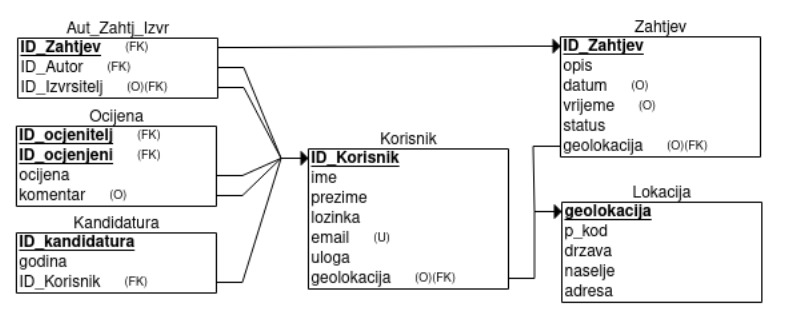
\includegraphics[scale=0.65]{slike/dijagram2.jpeg} %veličina slike u odnosu na originalnu datoteku i pozicija slike
				\centering
				\caption \newline E-R dijagram baze podataka
				\label{fig:promjene}
			\end{figure}
			
			\eject
			
			
		\section{Dijagram razreda}
		
			\textit{Potrebno je priložiti dijagram razreda s pripadajućim opisom. Zbog preglednosti je moguće dijagram razlomiti na više njih, ali moraju biti grupirani prema sličnim razinama apstrakcije i srodnim funkcionalnostima.}\\
			
			\textbf{\textit{dio 1. revizije}}\\
			
			\textit{Prilikom prve predaje projekta, potrebno je priložiti potpuno razrađen dijagram razreda vezan uz \textbf{generičku funkcionalnost} sustava. Ostale funkcionalnosti trebaju biti idejno razrađene u dijagramu sa sljedećim komponentama: nazivi razreda, nazivi metoda i vrste pristupa metodama (npr. javni, zaštićeni), nazivi atributa razreda, veze i odnosi između razreda.}\\
			
			\textbf{\textit{dio 2. revizije}}\\			
			
			\textit{Prilikom druge predaje projekta dijagram razreda i opisi moraju odgovarati stvarnom stanju implementacije}
			
			
			
			\eject
		
		\section{Dijagram stanja}
			
			
			\textbf{\textit{dio 2. revizije}}\\
			
			\textit{Potrebno je priložiti dijagram stanja i opisati ga. Dovoljan je jedan dijagram stanja koji prikazuje \textbf{značajan dio funkcionalnosti} sustava. Na primjer, stanja korisničkog sučelja i tijek korištenja neke ključne funkcionalnosti jesu značajan dio sustava, a registracija i prijava nisu. }
			
			
			\eject 
		
		\section{Dijagram aktivnosti}
			
			\textbf{\textit{dio 2. revizije}}\\
			
			 \textit{Potrebno je priložiti dijagram aktivnosti s pripadajućim opisom. Dijagram aktivnosti treba prikazivati značajan dio sustava.}
			
			\eject
		\section{Dijagram komponenti}
		
			\textbf{\textit{dio 2. revizije}}\\
		
			 \textit{Potrebno je priložiti dijagram komponenti s pripadajućim opisom. Dijagram komponenti treba prikazivati strukturu cijele aplikacije.}
	\chapter{Implementacija i korisničko sučelje}
		
		\section{Korištene tehnologije i alati}
		
			%\textbf{\textit{dio 2. revizije}}\\
			
            Komunikacija u timu realizirana je korištenjem aplikacije\underline{ Discord}\footnote{\url{https://discord.com/}},\underline{ MicrosoftTeams}\footnote{\url{https://www.microsoft.com/en-us/microsoft-365/microsoft-teams}} i \underline{WhatsApp}\footnote{\url{https://www.whatsapp.com/}}. Za izradu UML dijagrama korišten je alat \underline{Astah Professional}\footnote{\url{https://astah.net/}}, a kao sustav za upravljanje izvornim kodom \underline{Git}\footnote{\url{https://git-scm.com/}}. Udaljeni repozitorij projekta je dostupan na web platformi \underline{GitLab}\footnote{\url{https://about.gitlab.com/}}.
            Kao razvojno okruženje korišteni su \underline{IntelliJ}
            \footnote{\url{https://www.jetbrains.com/idea/}} - integrirano razvojno okruženje (IDE) tvrtke JetBrains.
            \underline{Spring Tool Suite}
            \footnote{\url{https://spring.io/tools}} (Eclipse) - integrirano razvojno okruženje namijenjeno za razvoj aplikacija koje koriste Spring kao radni okvir te \underline{VSCode}\footnote{\url{https://code.visualstudio.com/}} - integrirano razvojno okruženje pogodno za razvoj frontend-a.
            
            Aplikacija je napisana koristeći  radni
            okvir \underline{Spring Boot}\footnote{\url{https://spring.io/projects/spring-boot}} i jezik \underline{Javu}\footnote{\url{https://www.java.com/}} za
            izradu \emph{backenda} te \underline{React}\footnote{\url{https://reactjs.org/}} i jezik \underline{JavaScript}\footnote{\url{https://www.javascript.com/}} za izradu \emph{frontenda}.
            Spring Boot je open-source Javin radni okvir koji omogućuje izgradnju mikro servisa. Sam Spring Boot dolazi s već predkonfiguriranim značajkama koje programerima omogućuju konvencijonalnost te mogućnost pokretanja aplikacije bez dodatnog posla. 
            React, također poznat kao React.js ili ReactJS, je biblioteka u JavaScriptu za izgradnju korisničkih
            sučelja. Složene aplikacije u React-u obično zahtijevaju korištenje dodatnih biblioteka za interakciju s API-jem.
            
            Baza podataka i aplikacija se nalaze na poslužitelju \underline{Heroku}
            \footnote{\url{https://www.heroku.com/}}.
            
        
\newpage 

\begin{comment}   
        \section{Ispitivanje programskog rješenja}
			
			\textbf{\textit{dio 2. revizije}}
			
			Svi testovi izvršeni su pomoću Junit i Selenium. Ispitivanje se radilo po obrascima uporabe kako bi
            se provjerila osnovna funkcionalnost sustava, ali i nasumičnim kretanjima po aplikaciji
            kako bi se pronašle neočekivane greške  ili nepredvidena ponašanja.
            Svaki dio sustava je ispitan, no zbog jednostavnosti u dokumentaciji će biti prikazan
            samo dio ispitivanja. Prikazivanje ispitivanja UC?, UC?, UC?,UC?, UC? i UC?.
            
\end{comment}

		    \section{Ispitivanje programskog rješenja}
			
			\textbf{\textit{dio 2. revizije}}\\
			
			 \textit{U ovom poglavlju je potrebno opisati provedbu ispitivanja implementiranih funkcionalnosti na razini komponenti i na razini cijelog sustava s prikazom odabranih ispitnih slučajeva. Studenti trebaju ispitati temeljnu funkcionalnost i rubne uvjete.}
           
%\begin{comment}
        \subsection{Ispitivanje komponenti}
		    
		    \textbf{\textit{dio 2. revizije}}\\
    
			\textit{Potrebno je provesti ispitivanje jedinica (engl. unit testing) nad razredima koji implementiraju temeljne funkcionalnosti. Razraditi \textbf{minimalno 6 ispitnih slučajeva} u kojima će se ispitati redovni slučajevi, rubni uvjeti te izazivanje pogreške (engl. exception throwing). Poželjno je stvoriti i ispitni slučaj koji koristi funkcionalnosti koje nisu implementirane. Potrebno je priložiti izvorni kôd svih ispitnih slučajeva te prikaz rezultata izvođenja ispita u razvojnom okruženju (prolaz/pad ispita). }
			
			
			
			\subsection{Ispitivanje sustava}
			
			 \textit{Potrebno je provesti i opisati ispitivanje sustava koristeći radni okvir Selenium\footnote{\url{https://www.seleniumhq.org/}}. Razraditi \textbf{minimalno 4 ispitna slučaja} u kojima će se ispitati redovni slučajevi, rubni uvjeti te poziv funkcionalnosti koja nije implementirana/izaziva pogrešku kako bi se vidjelo na koji način sustav reagira kada nešto nije u potpunosti ostvareno. Ispitni slučaj se treba sastojati od ulaza (npr. korisničko ime i lozinka), očekivanog izlaza ili rezultata, koraka ispitivanja i dobivenog izlaza ili rezultata.\\ }
			 
			 \textit{Izradu ispitnih slučajeva pomoću radnog okvira Selenium moguće je provesti pomoću jednog od sljedeća dva alata:}
			 \begin{itemize}
			 	\item \textit{dodatak za preglednik \textbf{Selenium IDE} - snimanje korisnikovih akcija radi automatskog ponavljanja ispita	}
			 	\item \textit{\textbf{Selenium WebDriver} - podrška za pisanje ispita u jezicima Java, C\#, PHP koristeći posebno programsko sučelje.}
			 \end{itemize}
		 	\textit{Detalji o korištenju alata Selenium bit će prikazani na posebnom predavanju tijekom semestra.}
			
			\eject 
%\end{comment}
\section{Dijagram razmještaja}
	
	\textbf{\textit{dio 2. revizije}}
	
	\text Dijagrami razmještaja opisuju topologiju sklopovlja i programsku potporu koja se koristi u implementaciji sustava u njegovom radnom okruženju. Na poslužitelju
	(HerokuCloudServer) je postavljen Linux operacijski sustav te se na njemu nalaze HTTP Server i poslužitelj baze podataka . Klijenti koriste web preglednik na svom uređaju(PC ili mobitel) kako bi pristupili web aplikaciji.Sustav je baziran na arhitekturi ”klijent – poslužitelj”, a komunikacija izmedu računala korisnika (klijent, zaposlenik,vlasnik, administrator) i poslužitelja odvija se preko HTTP veze.  

    %unos slike
		\begin{figure}[H]
			\includegraphics[scale=0.5]{slike/Dijagram Razmještaja.png} %veličina slike u odnosu na originalnu datoteku i pozicija slike
			\centering
			\caption { Dijagram Razmještaja}
			\label{fig:5.1}
			\end{figure}


\begin{comment}	
	\textit{Potrebno je umetnuti \textbf{specifikacijski} dijagram razmještaja i opisati ga. Moguće je umjesto specifikacijskog dijagrama razmještaja umetnuti dijagram razmještaja instanci, pod uvjetom da taj dijagram bolje opisuje neki važniji dio sustava.}
	
	\eject 
\end{comment}

\newpage


\section{Upute za puštanje u pogon}

	\textbf{\textit{dio 2. revizije}}\\

	\textit{U ovom poglavlju potrebno je dati upute za puštanje u pogon (engl. deployment) ostvarene aplikacije. Na primjer, za web aplikacije, opisati postupak kojim se od izvornog kôda dolazi do potpuno postavljene baze podataka i poslužitelja koji odgovara na upite korisnika. Za mobilnu aplikaciju, postupak kojim se aplikacija izgradi, te postavi na neku od trgovina. Za stolnu (engl. desktop) aplikaciju, postupak kojim se aplikacija instalira na računalo. Ukoliko mobilne i stolne aplikacije komuniciraju s poslužiteljem i/ili bazom podataka, opisati i postupak njihovog postavljanja. Pri izradi uputa preporučuje se \textbf{naglasiti korake instalacije uporabom natuknica} te koristiti što je više moguće \textbf{slike ekrana} (engl. screenshots) kako bi upute bile jasne i jednostavne za slijediti.}
		
		
	\textit{Dovršenu aplikaciju potrebno je pokrenuti na javno dostupnom poslužitelju. Studentima se preporuča korištenje neke od sljedećih besplatnih usluga: \href{https://aws.amazon.com/}{Amazon AWS}, \href{https://azure.microsoft.com/en-us/}{Microsoft Azure} ili \href{https://www.heroku.com/}{Heroku}. Mobilne aplikacije trebaju biti objavljene na F-Droid, Google Play ili Amazon App trgovini.}
	
	
	\eject 


	\chapter{Zaključak i budući rad}
		
		\textbf{\textit{dio 2. revizije}}\\
		
		 \textit{U ovom poglavlju potrebno je napisati osvrt na vrijeme izrade projektnog zadatka, koji su tehnički izazovi prepoznati, jesu li riješeni ili kako bi mogli biti riješeni, koja su znanja stečena pri izradi projekta, koja bi znanja bila posebno potrebna za brže i kvalitetnije ostvarenje projekta i koje bi bile perspektive za nastavak rada u projektnoj grupi.}
		
		 \textit{Potrebno je točno popisati funkcionalnosti koje nisu implementirane u ostvarenoj aplikaciji.}
		
		\eject 
	\chapter*{Popis literature}
		\addcontentsline{toc}{chapter}{Popis literature}
	 	
 		\textbf{\textit{Kontinuirano osvježavanje}}
	
		\textit{Popisati sve reference i literaturu koja je pomogla pri ostvarivanju projekta.}
		
		
		\begin{enumerate}
			
			
			\item  Programsko inženjerstvo, FER ZEMRIS, \url{http://www.fer.hr/predmet/proinz}
			
			\item  I. Sommerville, "Software engineering", 8th ed, Addison Wesley, 2007.
			
			\item  T.C.Lethbridge, R.Langaniere, "Object-Oriented Software Engineering", 2nd ed. McGraw-Hill, 2005.
			
			\item  I. Marsic, Software engineering book``, Department of Electrical and Computer Engineering, Rutgers University, \url{http://www.ece.rutgers.edu/~marsic/books/SE}
			
			\item  The Unified Modeling Language, \url{https://www.uml-diagrams.org/}
			
			\item  Astah Community, \url{http://astah.net/editions/uml-new}
		\end{enumerate}
		
		 
	
	
	\begingroup
	\renewcommand*\listfigurename{Indeks slika i dijagrama}
	%\renewcommand*\listtablename{Indeks tablica}
	%\let\clearpage\relax
	\listoffigures
	%\vspace{10mm}
	%\listoftables
	\endgroup
	\addcontentsline{toc}{chapter}{Indeks slika i dijagrama}

	
	\eject 
		
	\chapter*{Dodatak: Prikaz aktivnosti grupe}
		\addcontentsline{toc}{chapter}{Dodatak: Prikaz aktivnosti grupe}
		
		\section*{Dnevnik sastajanja}
		
		
		\begin{packed_enum}
			\item  sastanak
			
			\item[] \begin{packed_item}
				\item Datum: 2. listopada 2020.
				\item Prisustvovali: I.Bokšić, I.Jakas, M.Lipovac, M.Oreč, J.Roček, R.Đaković, D.Ćurić
				\item Teme sastanka:
				\begin{packed_item}
					\item  upoznavanje tima
					\item  razgovor o projektu i trenutnim tehnološkim znanjima članova
				\end{packed_item}
			\end{packed_item}
			
				\item  sastanak
			\item[] \begin{packed_item}
				\item Datum: 8. listopada 2020.
				\item Prisustvovali: I.Bokšić, I.Jakas, M.Lipovac, M.Oreč, J.Roček, R.Đaković, D.Ćurić
				\item Teme sastanka:
				\begin{packed_item}
					\item  razgovor s asistenticom i demostratorom
					\item analiza projekta
					\item razješavanje prvih nedoumica oko zadatka 
				\end{packed_item}
			\end{packed_item}
		
			\item  sastanak
			\item[] \begin{packed_item}
				\item Datum: 10. listopada 2020.
				\item Prisustvovali: I.Bokšić, I.Jakas, M.Lipovac, M.Oreč, J.Roček, R.Đaković, D.Ćurić
				\item Teme sastanka:
				\begin{packed_item}
					\item  razgovor o tehnologijama koje ćemo koristiti i njihova instalacija
					\item  okvirna podjela rada
				\end{packed_item}
			\end{packed_item}
			
			
				\item  sastanak
			\item[] \begin{packed_item}
				\item Datum: 14. listopada 2020.
				\item Prisustvovali: I.Bokšić, I.Jakas, M.Lipovac, M.Oreč, J.Roček, R.Đaković, D.Ćurić
				\item Teme sastanka:
				\begin{packed_item}
					\item definiranje funkcionalnih zahtjeva 
					\item kreiranje use case dijagrama
				\end{packed_item}
			\end{packed_item}
			%
				\item  sastanak
			\item[] \begin{packed_item}
				\item Datum: 16. listopada 2020.
				\item Prisustvovali: I.Bokšić, M.Lipovac, M.Oreč, J.Roček, R.Đaković, D.Ćurić
				\item Teme sastanka:
				\begin{packed_item}
					\item konačno definiranje use case dijagrama
					\item nova podjela zadataka
				\end{packed_item}
			\end{packed_item}
			%
	
		\item  sastanak
		\item[] \begin{packed_item}
			\item Datum:  26. listopada 2020.
			\item Prisustvovali: D.Ćurić
			\item Teme sastanka:
			\begin{packed_item}
				\item razgovor s asistenticom i demostratorom
				\item rasprava o sekvencijskim dijagramima
			\end{packed_item}
		\end{packed_item}
		%

			\item  sastanak
		\item[] \begin{packed_item}
			\item Datum: 3. studenog 2020.
			\item Prisustvovali: I.Bokšić, M.Lipovac, R.Đaković, D.Ćurić
			\item Teme sastanka:
			\begin{packed_item}
				\item raspodijela posla na dokumentaciji 
				\item prezentiranje login i  sign in stranice  
			\end{packed_item}
		\end{packed_item}
		%
		
			\item  sastanak
		\item[] \begin{packed_item}
			\item Datum: 3. studenog 2020.
			\item Prisustvovali: J.Roček
			\item Teme sastanka:
			\begin{packed_item}
				\item razgovor s demonstratorom  
				\item rasprava oko implementacije JWT-a 
			\end{packed_item}
		\end{packed_item}
		%
		
			\item  sastanak
		\item[] \begin{packed_item}
			\item Datum: 5. studenog 2020.
			\item Prisustvovali: I.Bokšić, I.Jakas, M.Lipovac, M.Oreč, J.Roček, R.Đaković, D.Ćurić
			\item Teme sastanka:
			\begin{packed_item}
				\item razgovor s asistenticom i demostratorom
				\item komentiranje dijagrama baze podataka
				\item sugestija oko izrade dijagrama razreda
			\end{packed_item}
		\end{packed_item}
		%
		
		  \item  sastanak
		\item[] \begin{packed_item}
			\item Datum: 10. prosinca 2020.
			\item Prisustvovali: J.Roček, D.Ćurić, M.Oreč, M.Lipovac
			\item Teme sastanka:
			\begin{packed_item}
				\item dogovor oko implementacijskih detalja vezanih
				     uz backend
			\end{packed_item}
		\end{packed_item}
		%
		
			\item  sastanak
		\item[] \begin{packed_item}
			\item Datum: 15. prosinac 2020.
			\item Prisustvovali:J.Roček, D.Ćurić 
			\item Teme sastanka:
			\begin{packed_item}
				\item pregled napravljenih dijelova backend
				\item definiranje novih zadataka za backend
				
			\end{packed_item}
		\end{packed_item}
		%
		
			\item  sastanak
		\item[] \begin{packed_item}
			\item Datum: 17. prosinca 2020.
			\item Prisustvovali: J.Roček, M.Oreč, M.Lipovac 
			\item Teme sastanka:
			\begin{packed_item}
				\item pregled napravljenih dijelova backend
			    \item definiranje novih zadataka za backend
			\end{packed_item}
		\end{packed_item}
		%
		
			\item  sastanak
		\item[] \begin{packed_item}
			\item Datum: 22. prosinca 2020.
			\item Prisustvovali: J.Roček, D.Ćurić 
			\item Teme sastanka:
			\begin{packed_item}
				\item pregled napravljenih dijelova backend
			    \item modificiranje postojećih metoda 
			    \item definiranje novih zadataka za backend
			\end{packed_item}
		\end{packed_item}
		%
		
		    \item  sastanak
		\item[] \begin{packed_item}
			\item Datum: 23. prosinca 2020.
			\item Prisustvovali: J.Roček, I.Jakas, R.Đaković, I.Bokšić
			\item Teme sastanka:
			\begin{packed_item}
				\item pregled napravljenih dijelova backend
			    \item definiranje zadataka za frontend
			\end{packed_item}
		\end{packed_item}
		%
		
		\item  sastanak
		\item[] \begin{packed_item}
			\item Datum: 27. prosinca 2020.
			\item Prisustvovali: I.Jakas, R.Đaković, I.Bokšić
			\item Teme sastanka:
			\begin{packed_item}
				\item pregled rada na frontu
				\item definiranje novih zadataka na frontu
			\end{packed_item}
		\end{packed_item}
		%
		
			\item  sastanak
		\item[] \begin{packed_item}
			\item Datum: 3. siječnja 2021.
			\item Prisustvovali: J.Roček, M.Oreč, M.LIpovac
			\item Teme sastanka:
			\begin{packed_item}
				\item dogovor oko pisanja JUnit testova
			    \item dogovor oko same implementacije JUnit testova
			\end{packed_item}
		\end{packed_item}
		%
		
		\item  sastanak
		\item[] \begin{packed_item}
			\item Datum: 4. siječnja 2020.
			\item Prisustvovali: I.Jakas, R.Đaković, I.Bokšić, J.Roček
			\item Teme sastanka:
			\begin{packed_item}
				\item pregled fronta 
				\item novo definiranje zadataka
			\end{packed_item}
		\end{packed_item}
		%
		
		\item  sastanak
		\item[] \begin{packed_item}
			\item Datum: 7. siječnja 2020.
			\item Prisustvovali: I.Jakas, R.Đaković, I.Bokšić, J.Roček, M.Lipovac, M.Oreč, D.Ćurić
			\item Teme sastanka:
			\begin{packed_item}
				\item demonstriranje alfa verzije asistentici 
				\item popravci funkcionalnosti
			\end{packed_item}
		\end{packed_item}
		%
		
		\item  sastanak
		\item[] \begin{packed_item}
			\item Datum: 13. siječnja 2021.
			\item Prisustvovali: J.Roček, R.Đaković, I. Bokšić
			\item Teme sastanka:
			\begin{packed_item}
				\item konačni pregled aplikacije i popravci
				\item rasprava oko dokumentacije
			\end{packed_item}
		\end{packed_item}
		%
		
	\end{packed_enum}

		
		
		\eject
		\section*{Tablica aktivnosti}
		
		%	\textbf{\textit{Kontinuirano osvježavanje}}\\
			
		%	 \textit{Napomena: Doprinose u aktivnostima treba navesti u satima po članovima grupe po aktivnosti.}
					
						
			
			\begin{longtabu} to \textwidth {|X[7, l]|X[1, c]|X[1, c]|X[1, c]|X[1, c]|X[1, c]|X[1, c]|X[1, c]|}
								
				\cline{2-8} \multicolumn{1}{c|}{\textbf{}} &     
				\multicolumn{1}{c|}{\rotatebox{90}{\textbf{Iva Bokšić }}} & \multicolumn{1}{c|}{\rotatebox{90}{\textbf{Jan Roček }}} &	\multicolumn{1}{c|}{\rotatebox{90}{\textbf{Ivan Jakas }}} &	\multicolumn{1}{c|}{\rotatebox{90}{\textbf{Robert Đaković }}} &
				\multicolumn{1}{c|}{\rotatebox{90}{\textbf{Matea Lipovac}}} &
				\multicolumn{1}{c|}{\rotatebox{90}{\textbf{Dominik Ćurić }}} &	\multicolumn{1}{c|}{\rotatebox{90}{\textbf{Marija Oreč }}} \\ \hline 
				\endfirsthead
				
			
				\cline{2-8} \multicolumn{1}{c|}{\textbf{}} &     
				\multicolumn{1}{c|}{\rotatebox{90}{\textbf{Iva Bokšić }}} & \multicolumn{1}{c|}{\rotatebox{90}{\textbf{Jan Roček }}} &	\multicolumn{1}{c|}{\rotatebox{90}{\textbf{Ivan Jakas }}} &	\multicolumn{1}{c|}{\rotatebox{90}{\textbf{Robert Đaković }}} &
				\multicolumn{1}{c|}{\rotatebox{90}{\textbf{Matea Lipovac}}} &
				\multicolumn{1}{c|}{\rotatebox{90}{\textbf{Dominik Ćurić }}} &	\multicolumn{1}{c|}{\rotatebox{90}{\textbf{Marija Oreč }}} \\ \hline 
				\endhead
				
				
				\endfoot
							
				 
				\endlastfoot
				
				Upravljanje projektom 		&2  &3  &2  &1  &  &  & \\ \hline
				Opis projektnog zadatka 	&  &  &  &  &  &  &5 \\ \hline
				
				Funkcionalni zahtjevi       &1  &1  &1  &1  &1  &1  &1  \\ \hline
				Opis pojedinih obrazaca 	&4  &   &  &  &6  &  &  \\ \hline
				Dijagram obrazaca 			&2  &3  &  &1  &  &1  &2  \\ \hline
				Sekvencijski dijagrami 		&  &  &2  &2  &  &5  &  \\ \hline
				Opis ostalih zahtjeva 		&  &  &  &  &  &  &1  \\ \hline

				Arhitektura i dizajn sustava	 &4  &2  &  &  &  &  &  \\ \hline
				Baza podataka				&2  &5  &  &  &1  &1  &   \\ \hline
				Dijagram razreda 			&1  &  &  &  &2  &  &3   \\ \hline
				Dijagram stanja				&  &  &  &  &  &7  &  \\ \hline
				Dijagram aktivnosti 		&  &  &  &  &  &4  &  \\ \hline
				Dijagram komponenti			&  &  &  &  &  &4  &  \\ \hline
				Korištene tehnologije i alati 		&  &  &  &  &  &1  &  \\ \hline
				Ispitivanje programskog rješenja 	&  &1  &  &  &10  &  &10  \\ \hline
				Dijagram razmještaja			&  &  &  &  &  &1  &  \\ \hline
				Upute za puštanje u pogon 		&1  &1  &  &  &  &  &  \\ \hline 
				Dnevnik sastajanja 			&1  &  &  &  &  &1  &  \\ \hline
				Zaključak i budući rad 		&  &  &  &  &2  &  &2  \\  \hline
				Popis literature 			&1  &  &  &  &  &  &  \\  \hline
				Izrada login stranice			&1  &  &3  &1  &  &  &  \\ \hline 
				Izrada baze podataka 		 			&1  &2  &  &  &  &  & \\ \hline 
				Integriranje fronta i backa 	&  &15  &  &  &  &  &  \\ \hline
				Backend							&  &100  &  &  &20  &20  &20  \\  \hline
				Front							&50  &10  &70  &60  &  &  &  \\  \hline
				 							
				
				
			\end{longtabu}
				
			
			\eject
			\section*{Dijagrami pregleda promjena}
			
		
			
		%	\textit{Prenijeti dijagram pregleda promjena nad datotekama projekta. Potrebno je na kraju projekta generirane grafove s gitlaba prenijeti u ovo poglavlje dokumentacije. Dijagrami za vlastiti projekt se mogu preuzeti s gitlab.com stranice, u izborniku Repository, pritiskom na stavku Contributors.}
		
		\begin{figure}[H]
			\begin{center}
				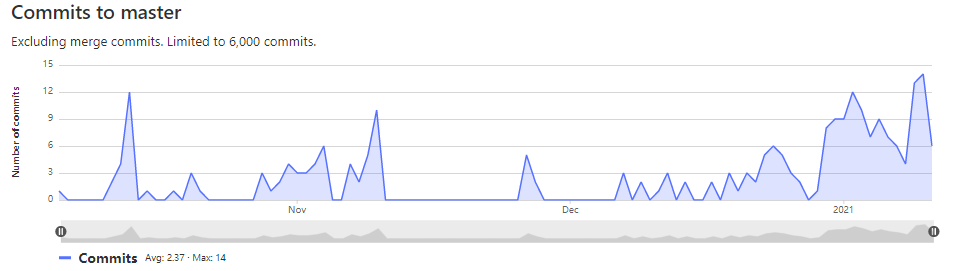
\includegraphics[width=15cm]{slike/master.png}
			\end{center}
			\caption{Dijagram pregleda promjena na grani master}
			\label{fig:master}
		\end{figure}
		
		\begin{figure}[H]
			\begin{center}
				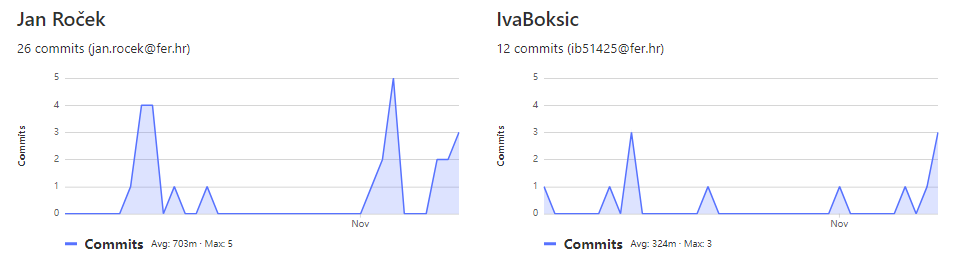
\includegraphics[width=15cm]{slike/master1.PNG}
				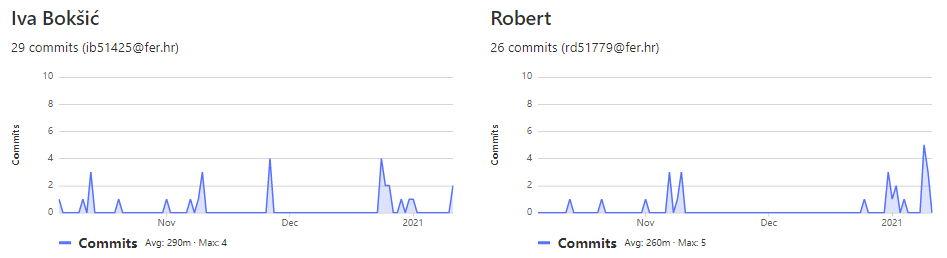
\includegraphics[width=15cm]{slike/master2.PNG}
				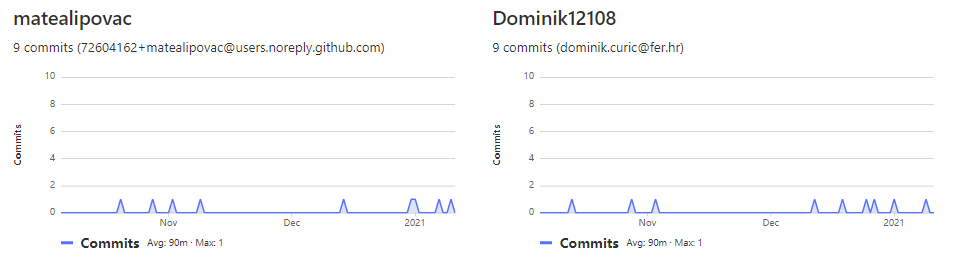
\includegraphics[width=15cm]{slike/master3.PNG}
				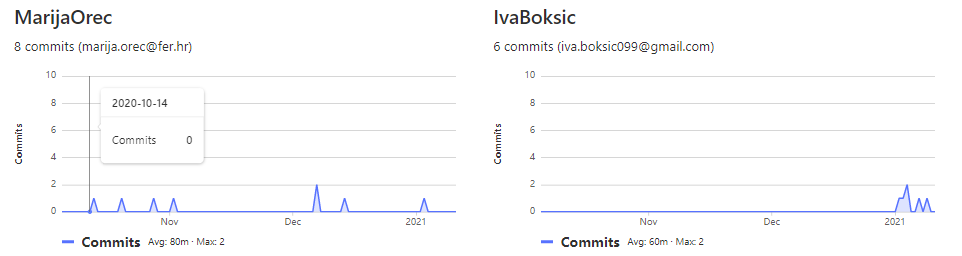
\includegraphics[width=15cm]{slike/master4.PNG}
				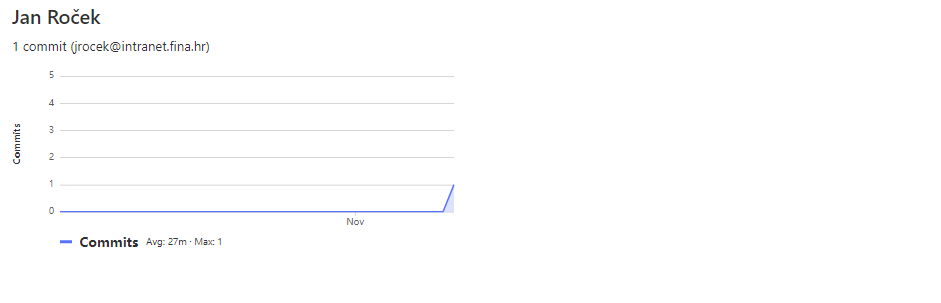
\includegraphics[width=15cm]{slike/master5.PNG}
			\end{center}
			\label{fig:dijapre}
		\end{figure}
	
	


\end{document} %naredbe i tekst nakon ove naredbe ne ulaze u izgrađen dokument 


